% Soubory musí být v kódování, které je nastaveno v příkazu \usepackage[...]{inputenc}

\documentclass[%        Základní nastavení
  %draft,    				  % Testovací překlad
  12pt,       				% Velikost základního písma je 12 bodů
	t,                  % obsah slajdů bude vždy začínat od shora (nebude vertikálně centrovaný)
	aspectratio=1610,   % poměr stran bude 16:10 (všechny projektory v učebnách na Technické 12 Brno),
	                    % další volby jsou 43, 149, 169, 54, 32.
	unicode,						% Záložky a informace budou v kódování unicode
]{beamer}				    	% Dokument třídy 'zpráva', vhodná pro sazbu závěrečných prací s kapitolami
%\usepackage{etex}

\usepackage[utf8]		  % Kódování zdrojových souborů je v UTF-8
	{inputenc}					% Balíček pro nastavení kódování zdrojových souborů
	
\usepackage{graphicx} % Balíček 'graphicx' pro vkládání obrázků
											% Nutné pro vložení logotypů školy a fakulty

\usepackage[          % Balíček 'acronym' pro sazby zkratek a symbolů
	nohyperlinks				% Nebudou tvořeny hypertextové odkazy do seznamu zkratek
]{acronym}						
											% Nutné pro použití prostředí 'acronym' balíčku 'thesis'

%% Balíček hyperref je volán třídou beamer automaticky, proto není třeba následujícího kódu:
%\usepackage[
%	breaklinks=true,		% Hypertextové odkazy mohou obsahovat zalomení řádku
%	hypertexnames=false % Názvy hypertextových odkazů budou tvořeny
%											% nezávisle na názvech TeXu
%]{hyperref}						% Balíček 'hyperref' pro sazbu hypertextových odkazů
%											% Nutné pro použití příkazu 'nastavenipdf' balíčku 'thesis'

\usepackage{cmap} 		% Balíček cmap zajišťuje, že PDF vytvořené `pdflatexem' je
											% plně "prohledávatelné" a "kopírovatelné"

%\usepackage{upgreek}	% Balíček pro sazbu stojatých řeckých písmem
											%% např. stojaté pí: \uppi
											%% např. stojaté mí: \upmu (použitelné třeba v mikrometrech)
											%% pozor, grafická nekompatibilita s fonty typu Computer Modern!

%\usepackage{amsmath} %balíček pro sabu náročnější matematiky

\usepackage{booktabs} % Balíček, který umožňuje v tabulce používat
                      % příkazy \toprule, \midrule, \bottomrule


%%%%%%%%%%%%%%%%%%%%%%%%%%%%%%%%%%%%%%%%%%%%%%%%%%%%%%%%%%%%%%%%%
%%%%%%      Definice informací o dokumentu             %%%%%%%%%%
%%%%%%%%%%%%%%%%%%%%%%%%%%%%%%%%%%%%%%%%%%%%%%%%%%%%%%%%%%%%%%%%%

% V tomto souboru se nastavují téměř veškeré informace, proměnné mezi studenty:
% jméno, název práce, pohlaví atd.
% Tento soubor je SDÍLENÝ mezi textem práce a prezentací k obhajobě -- netřeba něco nastavovat na dvou místech.

\usepackage[
%%% Z následujících voleb jazyka lze použít pouze jednu
  czech-english,		% originální jazyk je čeština, překlad je anglicky (výchozí)
  %english-czech,	% originální jazyk je angličtina, překlad je česky
  %slovak-english,	% originální jazyk je slovenština, překlad je anglicky
  %english-slovak,	% originální jazyk je angličtina, překlad je slovensky
%
%%% Z následujících voleb typu práce lze použít pouze jednu
  semestral,		  % semestrální práce (výchozí)
  %bachelor,			%	bakalářská práce
  %master,			  % diplomová práce
  %treatise,			% pojednání o disertační práci
  %doctoral,			% disertační práce
%
%%% Z následujících voleb zarovnání objektů lze použít pouze jednu
%  left,				  % rovnice a popisky plovoucích objektů budou zarovnány vlevo
	center,			    % rovnice a popisky plovoucích objektů budou zarovnány na střed (vychozi)
%
]{thesis}   % Balíček pro sazbu studentských prací


%%% Jméno a příjmení autora ve tvaru
%  [tituly před jménem]{Křestní}{Příjmení}[tituly za jménem]
% Pokud osoba nemá titul před/za jménem, smažte celý řetězec '[...]'
\author[]{Jakub}{Charvot}

%%% Identifikační číslo autora (VUT ID)
\butid{240844}

%%% Pohlaví autora/autorky
% (nepoužije se ve variantě english-czech ani english-slovak)
% Číselná hodnota: 1...žena, 0...muž
\gender{0}

%%% Jméno a příjmení vedoucího/školitele včetně titulů
%  [tituly před jménem]{Křestní}{Příjmení}[tituly za jménem]
% Pokud osoba nemá titul před/za jménem, smažte celý řetězec '[...]'
\advisor[Ing.]{Pavel}{Tomíček}[]

%%% Jméno a příjmení oponenta včetně titulů
%  [tituly před jménem]{Křestní}{Příjmení}[tituly za jménem]
% Pokud osoba nemá titul před/za jménem, smažte celý řetězec '[...]'
% Nastavení oponenta se uplatní pouze v prezentaci k obhajobě;
% v případě, že nechcete, aby se na titulním snímku prezentace zobrazoval oponent, pouze příkaz zakomentujte;
% u obhajoby semestrální práce se oponent nezobrazuje (jelikož neexistuje)
% U dizertační práce jsou typicky dva až tři oponenti. Pokud je chcete mít na titulním slajdu, prosím ručně odkomentujte a upravte jejich jména v definici "VUT title page" v souboru thesis.sty.
\opponent[doc.]{Oponent}{Krutý}[Ph.D.]

%%% Název práce
%  Parametr ve složených závorkách {} je název v originálním jazyce,
%  parametr v hranatých závorkách [] je překlad (podle toho jaký je originální jazyk).
%  V případě, že název Vaší práce je dlouhý a nevleze se celý do zápatí prezentace, použijte příkaz
%  \def\insertshorttitle{Zkác.\ náz.\ práce}
%  kde jako parametr vyplníte zkrácený název. Pokud nechcete zkracovat název, budete muset předefinovat,
%  jak se vytváří patička slidu. Viz odkaz: https://bit.ly/3EJTp5A
\title[Autonomous aquarium]{Autonomní akvárium}

%%% Označení oboru studia
%  Parametr ve složených závorkách {} je název oboru v originálním jazyce,
%  parametr v hranatých závorkách [] je překlad
\specialization[Microelectronics and Technology]{Mikroelektronika a technologie}

%%% Označení ústavu
%  Parametr ve složených závorkách {} je název ústavu v originálním jazyce,
%  parametr v hranatých závorkách [] je překlad
%\department[Department of Control and Instrumentation]{Ústav automatizace a měřicí techniky}
%\department[Department of Biomedical Engineering]{Ústav biomedicínského inženýrství}
%\department[Department of Electrical Power Engineering]{Ústav elektroenergetiky}
%\department[Department of Electrical and Electronic Technology]{Ústav elektrotechnologie}
%\department[Department of Physics]{Ústav fyziky}
%\department[Department of Foreign Languages]{Ústav jazyků}
%\department[Department of Mathematics]{Ústav matematiky}
\department[Department of Microelectronics]{Ústav mikroelektroniky}
%\department[Department of Radio Electronics]{Ústav radioelektroniky}
%\department[Department of Theoretical and Experimental Electrical Engineering]{Ústav teoretické a experimentální elektrotechniky}
% \department[Department of Telecommunications]{Ústav telekomunikací}
%\department[Department of Power Electrical and Electronic Engineering]{Ústav výkonové elektrotechniky a elektroniky}

%%% Označení fakulty
%  Parametr ve složených závorkách {} je název fakulty v originálním jazyce,
%  parametr v hranatých závorkách [] je překlad
%\faculty[Faculty of Architecture]{Fakulta architektury}
\faculty[Faculty of Electrical Engineering and~Communication]{Fakulta elektrotechniky a~komunikačních technologií}
%\faculty[Faculty of Chemistry]{Fakulta chemická}
%\faculty[Faculty of Information Technology]{Fakulta informačních technologií}
%\faculty[Faculty of Business and Management]{Fakulta podnikatelská}
%\faculty[Faculty of Civil Engineering]{Fakulta stavební}
%\faculty[Faculty of Mechanical Engineering]{Fakulta strojního inženýrství}
%\faculty[Faculty of Fine Arts]{Fakulta výtvarných umění}
%
%Nastavení logotypu (v hranatych zavorkach zkracene logo, ve slozenych plne):
\facultylogo[logo/FEKT_zkratka_barevne_PANTONE_CZ]{logo/UTKO_color_PANTONE_CZ}

%%% Rok odevzdání práce
\graduateyear{2024}
%%% Akademický rok odevzdání práce
\academicyear{2023/24}

%%% Datum obhajoby (uplatní se pouze v prezentaci k obhajobě)
\date{11.\,11.\,1980} 

%%% Místo obhajoby
% Na titulních stránkách bude automaticky vysázeno VELKÝMI písmeny (pokud tyto stránky sází šablona)
\city{Brno}

%%% Abstrakt
\abstract[%
This thesis delves into the topic of~aquarium automation, aiming to~design custom device for this purpose. A~market survey is~presented with depiction of~existing commercial solutions in~the~field of~automation, also the~essential technology requirements for~efficient aquarium operation are summarized. Regarding the~design of~the~custom device, the~thesis explain the~chosen architecture and takes a~deeper look at~some of~its~parts. The main outcome of~this thesis is the~creation of~an~electrical schematic for the~control unit. The~present work will be followed by a bachelor's thesis, within which the~device will be completed.
]{%
Tato práce se zaměřuje na problematiku automatizace akvárií a jejím cílem je navrhnout vlastní zařízení sloužící tomuto účelu. V práci je proveden trůzkum trhu a popsána již existující komerční řešení věnující se právě automatizaci, také je zde obsaženo shrnutí minimální techniky potřebné pro provoz akvária. Z hlediska návrhu vlastního zařízení je obsažen popis a odůvodnění zvolené architektury, dále se text detailněji věnuje některým dílčím blokům. Výstupem práce je zejména navržené elektrické schéma řídící jednotky. Na tuto práci bude navazovat bakalářská práce, v rámci které bude zařízení dokončeno. 
}

%%% Klíčová slova
\keywrds[%
aquaristics, automation, ESP32, data buses, device design
]{%
akvaristika, automatizace, ESP32, sběrnice, návrh zařízení
}


%%% Poděkování
\acknowledgement{%
Rád bych poděkoval vedoucímu semestrální práce
panu Ing.~Pavlu Tomíčkovi\ za ochotu i trpělivost, kterou se mnou měl po celou dobu tvorby této práce, a za mnoho cenných a podnětných rad k její odborné i formální stránce. Dále děkuji svému kamarádovi Radku Jančičkovi za osvětu v oblasti akvaristiky. 

}%      % v tomto souboru doplňte údaje o sobě, o názvu práce...
                       % (tento soubor je sdílený s textem práce)





%%%%%%%%%%%%%%%%%%%%%%%%%%%%%%%%%%%%%%%%%%%%%%%%%%%%%%%%%%%%%%%%%%%%%%%%

%%%%%%%%%%%%%%%%%%%%%%%%%%%%%%%%%%%%%%%%%%%%%%%%%%%%%%%%%%%%%%%%%%%%%%%%
%%%%%%     Nastavení polí ve Vlastnostech dokumentu PDF      %%%%%%%%%%%
%%%%%%%%%%%%%%%%%%%%%%%%%%%%%%%%%%%%%%%%%%%%%%%%%%%%%%%%%%%%%%%%%%%%%%%%
%% Při vloženém balíčku 'hyperref' lze použít příkaz '\pdfsettings'
\pdfsettings
%  Nastavení polí je možné provést také ručně příkazem:
%\hypersetup{
%  pdftitle={Název studentské práce},    	% Pole 'Document Title'
%  pdfauthor={Autor studenstké práce},   	% Pole 'Author'
%  pdfsubject={Typ práce}, 						  	% Pole 'Subject'
%  pdfkeywords={Klíčová slova}           	% Pole 'Keywords'
%}
\hypersetup{pdfpagemode=FullScreen}       % otevření rovnou v režimu celé obrazovky
%%%%%%%%%%%%%%%%%%%%%%%%%%%%%%%%%%%%%%%%%%%%%%%%%%%%%%%%%%%%%%%%%%%%%%%

\usetheme{VUT} 				% barvy a rozložení prezentace odpovídající VUT FEKT
% alternativně lze použít jiná berevná témata, ale bez záruky. Například: 
%\usetheme{Darmstadt} \usecolortheme{default2}
\logoheader					% vytvoření zkráceného loga VUT FEKT v hlavičce slajdu, nechte odkomentované




					   %%%%%%%%%%%%%%%%%%%%%%%%%%%%%%%%%%%%%%%%%%%%%%%%%%%%%%%%%%%%%%%%%
%%%%%%      !!! VLASTNÍ BALÍČKY A NASTAVENÍ !!!        %%%%%%%%%%
%%%%%%%%%%%%%%%%%%%%%%%%%%%%%%%%%%%%%%%%%%%%%%%%%%%%%%%%%%%%%%%%%
%====== Units =====
% \usepackage{siunitx}
% \sisetup{inter-unit-product =\ensuremath{\cdot}}
% \sisetup{group-digits = integer}
% \sisetup{output-decimal-marker = {,}}
% \sisetup{exponent-product = \ensuremath{\cdot}}
% \sisetup{separate-uncertainty}
% \sisetup{tight-spacing = false}
% \DeclareSIUnit\permille{\text{\textperthousand}}
%\sisetup{scientific-notation = true}
%\sisetup{round-mode=places,round-precision=4}
%\sisetup{evaluate-expression}

%====== Hyperlinky ====== 
% \hypersetup{allbordercolors={1 1 1}}

%====== Obrazky ========
% \usepackage{graphicx} 
% \usepackage[dvipsnames]{xcolor} % E: option clash for package xcolor
% \usepackage{tikz}

% ^^ už tam někde prý jsou použité

\usepackage[siunitx]{circuitikz}
% \usepackage{pgf}
% \usetikzlibrary{matrix}
\usetikzlibrary{fit}
% \usetikzlibrary{patterns}
% \usepackage{tkz-euclide}
% \usetikzlibrary{arrows.meta, bending, patterns.meta, ducks}
% \usetikzlibrary{shapes, backgrounds, decorations.pathmorphing, calc}
\usetikzlibrary{positioning}

% % \usepackage{derivative} % nebude potřeba 

% \usepackage{pgfplots}
% \pgfplotsset{width=0.8\linewidth, compat=1.17}
% \def\plotcscale{0.8}
% \usepackage{pgfplotstable}
% \newcommand*\circled[1]{\tikz[baseline=(char.base)]{
%             \node[shape=circle,draw,inner sep=1pt] (char) {#1};}}

% \usepackage[style=iso-numeric,backend=biber]{biblatex}
% \addbibresource{text/literatura.bib}
%making everything to match Juice citations
% \DeclareFieldFormat{labelnumberwidth}{\mkbibbrackets{#1}}
% \usepackage{natbib}
% \usepackage{url}
% \DeclareUrlCommand\url{\def\UrlLeft{<}\def\UrlRight{>} \urlstyle{tt}}


% TEMP
\usepackage{multirow}
\usepackage{array}
\usepackage{tabularx}
\usepackage{calc}


\begin{document}

% v případě zakomentování následujícího se zobrazí v pravém dolním rohu slajdů klikatelné navigační symboly 
\disablenavigationsymbols

% titulní snímek, vysazen bez horních, dolních a postranních lišt (volba plain),
% není tak vysazen ani nadpis snímku
\maketitle

%%%%%%%%%%%%%%%%%%%%%%%%%%%%%%%%%%%%%%%%%%%%%%%%%%%%%%%%%%%%%%%%%%%%%%%
% 1. snímek s cíli (zadaním) práce
\begin{frame} 
	% nadpis snímku
	\frametitle{Cíle práce}
	\begin{itemize}
			\item Navrhnout zařízení pro automatické monitorování a řízení akvária
			\item Průzkum trhu
				\begin{itemize}
					\item Používaná akvaristická technika 
					\item Existující řešení automatizace
					\begin{itemize}
						\item Cena 
						\item Rozsah funkcí
					\end{itemize}
				\end{itemize}
			\item Návrh vlastního zařízení
				\begin{itemize}
					\item Upřesnění požadavků
					\item Návrh architektury
					\item Tvorba schématu
				\end{itemize}
	\end{itemize}
\end{frame}

% region Vybavení akvária
%%%%%%%%%%%%% 1
% \begin{frame} 
% 	\frametitle{Vybavení akvária -- Požadavky}
	
% 	\begin{columns}[T] 								% prostředí sloupce s umístěním nahoře
% 		\begin{column}{0.4\textwidth}		% první sloupec
% 			Základní parametry:\\[2ex]
% 			%
% 			\begin{itemize}
% 				\item Velikost nádrže
% 				\item Sladká / slaná voda
% 			\end{itemize}
% 		\end{column}
% 		%
% 		\begin{column}{0.6\textwidth}		% druhý sloupec
% 			\begin{figure}%	
% 				\centering
% 				% \vspace{1cm}	              % horizontální mezera
% 				
\includegraphics[width=\columnwidth]{obrazky/prezentace/vybaveni-akvaria/01-prazdne.png}
% 				%lze vložit popisek, ale povetšinou je to v prezentaci zbytečné
% 				%\caption{Popisek obrázku}%
% 				%\label{obr:ukazka}
% 			\end{figure}
% 		\end{column}
% 	\end{columns}											% ukončení prostředí sloupce
% \end{frame}

%%%%%%%%%%%%% 2
% \begin{frame} 
% 	\frametitle{Vybavení akvária -- Požadavky}
	
% 	\begin{columns}[T] 								% prostředí sloupce s umístěním nahoře
% 		\begin{column}{0.4\textwidth}		% první sloupec
% 			Osazení:\\[2ex]
% 			%
% 			\begin{itemize}
% 				\item Každý druh má specifické požadavky
% 				\item Kompatibilita
% 			\end{itemize}
% 		\end{column}
% 		%
% 		\begin{column}{0.6\textwidth}		% druhý sloupec
% 			\begin{figure}%	
% 				\centering
% 				% \vspace{1cm}	              % horizontální mezera
% 				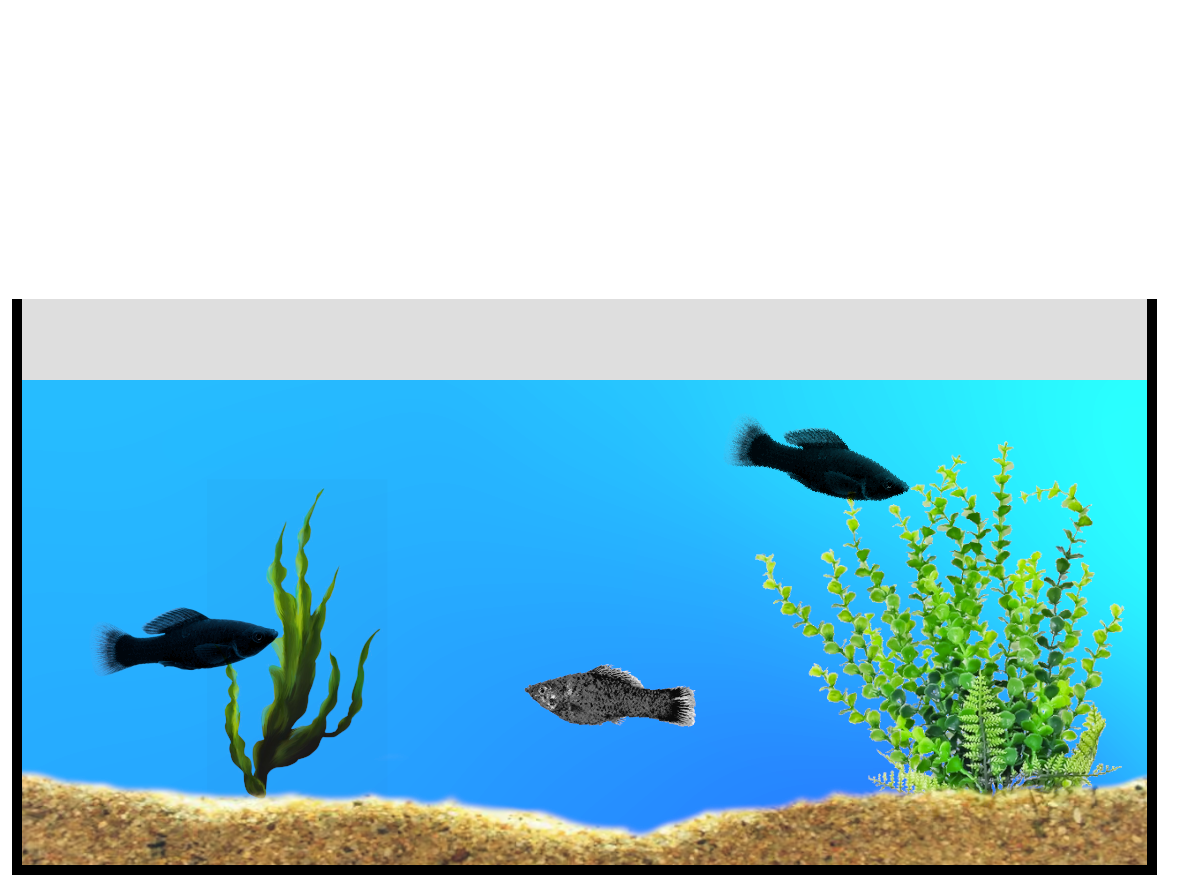
\includegraphics[width=\columnwidth]{obrazky/prezentace/vybaveni-akvaria/02-ryby-kytky}
% 				%lze vložit popisek, ale povetšinou je to v prezentaci zbytečné
% 				%\caption{Popisek obrázku}%
% 				%\label{obr:ukazka}
% 			\end{figure}
% 		\end{column}
% 	\end{columns}											% ukončení prostředí sloupce
% \end{frame}

%%%%%%%%%%%%%
% \begin{frame} 
% 	\frametitle{Vybavení akvária -- Filtrace vody}
	
% 	\begin{columns}[T] 								% prostředí sloupce s umístěním nahoře
% 		\begin{column}{0.4\textwidth}		% první sloupec
% 			Typy filtrů:\\[2ex]
% 			%
% 			\begin{itemize}
% 				\item Vnitřní / vnější filtr
% 			\end{itemize}

% 			\vspace{4ex}%
% 			Řízení:\\[2ex]
% 			%
% 			\begin{itemize}
% 				\item Kontinuální běh
% 				\item 230\,V
% 			\end{itemize}
% 		\end{column}
% 		%
% 		\begin{column}{0.6\textwidth}		% druhý sloupec
% 			\begin{figure}%	
% 				\centering
% 				% \vspace{1cm}	              % horizontální mezera
% 				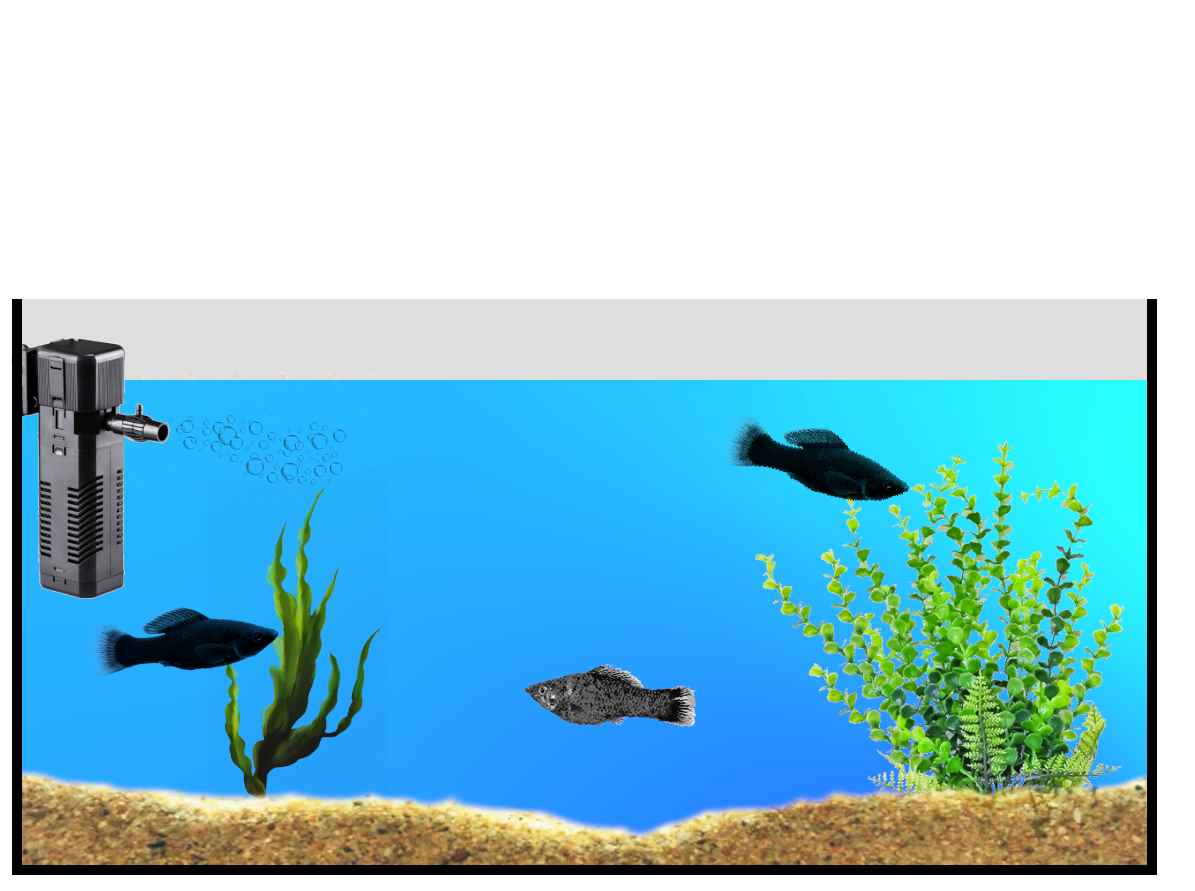
\includegraphics[width=\columnwidth]{obrazky/prezentace/vybaveni-akvaria/03-filtr.png}
% 				%lze vložit popisek, ale povetšinou je to v prezentaci zbytečné
% 				%\caption{Popisek obrázku}%
% 				%\label{obr:ukazka}
% 			\end{figure}
% 		\end{column}
% 	\end{columns}											% ukončení prostředí sloupce
% \end{frame}

%%%%%%%%%%%%%
% \begin{frame} 
% 	\frametitle{Vybavení akvária -- Osvětlení}
	
% 	\begin{columns}[T] 								% prostředí sloupce s umístěním nahoře
% 		\begin{column}{0.4\textwidth}		% první sloupec
% 			Typy:\\[2ex]
% 			%
% 			\begin{itemize}
% 				\item Zářivka
% 				\item Výbojka
% 				\item \acs{led} svítidlo
% 			\end{itemize}

% 			\vspace{4ex}%
% 			Řízení:\\[2ex]
% 			%
% 			\begin{itemize}
% 				\item Svícení během dne 
% 				\begin{itemize}
% 					\item Plynulý přechod (\acs{led})
% 				\end{itemize}
% 				\item 230\,V -- Zářivky a výbojky
% 				\item 0 až 5/12/24\,V -- \acs{led}
% 			\end{itemize}
% 		\end{column}
% 		%
% 		\begin{column}{0.6\textwidth}		% druhý sloupec
% 			\begin{figure}%	
% 				\centering
% 				% \vspace{1cm}	              % horizontální mezera
% 				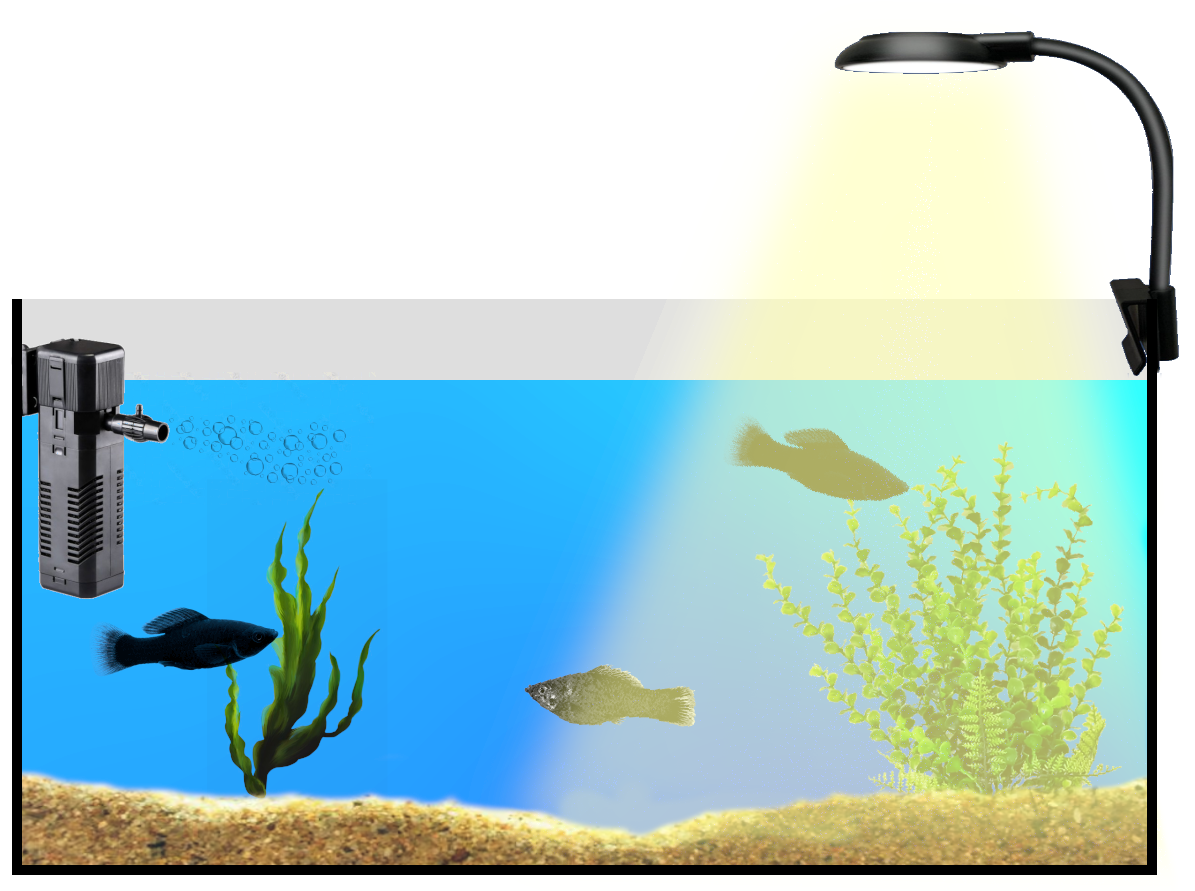
\includegraphics[width=\columnwidth]{obrazky/prezentace/vybaveni-akvaria/04-svetlo.png}
% 				%lze vložit popisek, ale povetšinou je to v prezentaci zbytečné
% 				%\caption{Popisek obrázku}%
% 				%\label{obr:ukazka}
% 			\end{figure}
% 		\end{column}
% 	\end{columns}											% ukončení prostředí sloupce
% \end{frame}

%%%%%%%%%%%%%
% \begin{frame} 
% 	\frametitle{Vybavení akvária -- Ohřev vody}
	
% 	\begin{columns}[T] 								% prostředí sloupce s umístěním nahoře
% 		\begin{column}{0.4\textwidth}		% první sloupec
% 			Typy:\\[2ex]
% 			%
% 			\begin{itemize}
% 				\item Ponorné odporové těleso
% 				\item Topný kabel
% 			\end{itemize}

% 			\vspace{4ex}%
% 			Řízení:\\[2ex]
% 			%
% 			\begin{itemize}
% 				\item Vlastní termostat 
% 				\item 230\,V
% 			\end{itemize}
% 		\end{column}
% 		%
% 		\begin{column}{0.6\textwidth}		% druhý sloupec
% 			\begin{figure}%	
% 				\centering
% 				% \vspace{1cm}	              % horizontální mezera
% 				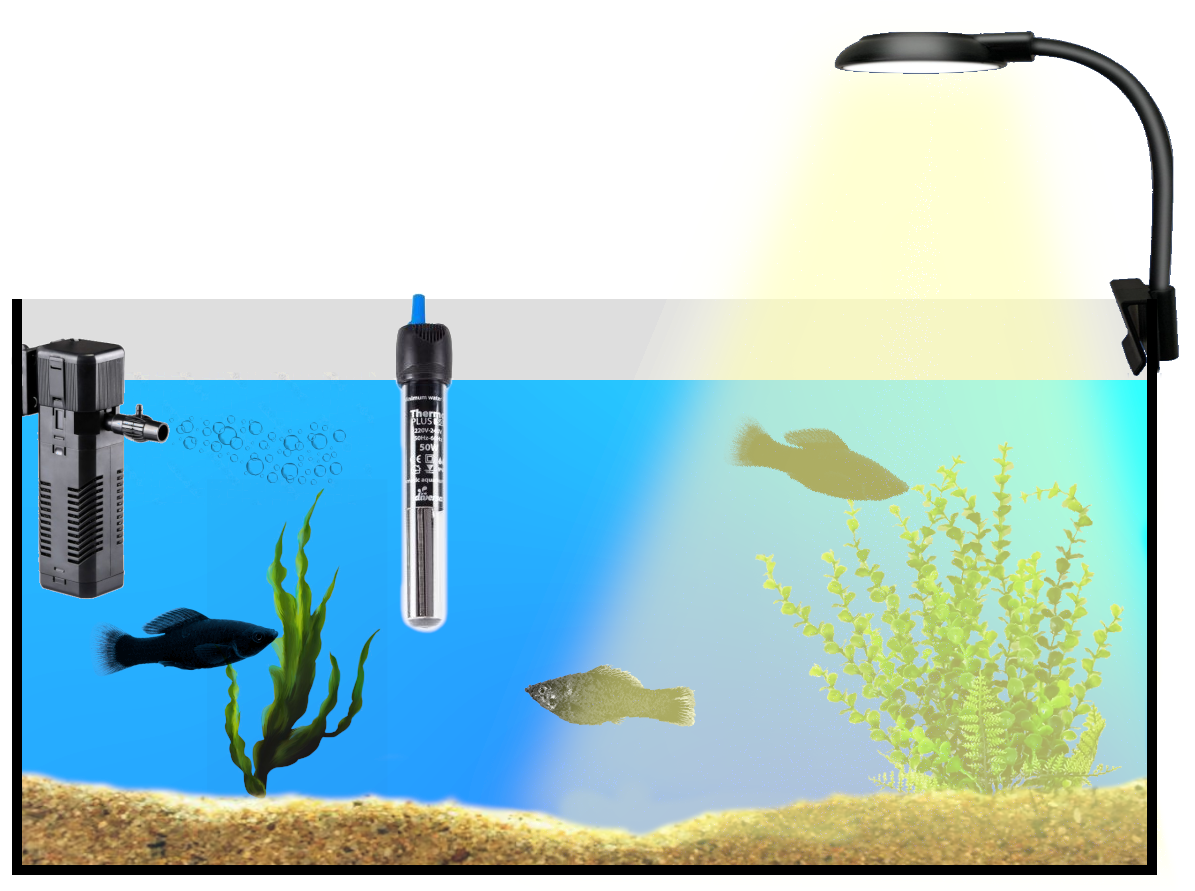
\includegraphics[width=\columnwidth]{obrazky/prezentace/vybaveni-akvaria/05-topeni.png}
% 				%lze vložit popisek, ale povetšinou je to v prezentaci zbytečné
% 				%\caption{Popisek obrázku}%
% 				%\label{obr:ukazka}
% 			\end{figure}
% 		\end{column}
% 	\end{columns}											% ukončení prostředí sloupce
% \end{frame}

%%%%%%%%%%%%%
\begin{frame} 
	\frametitle{Vybavení akvária}
	
	\begin{columns}[T] 								% prostředí sloupce s umístěním nahoře
		\begin{column}{0.4\textwidth}		% první sloupec
			Požadavky jsou určeny:\\[0ex]
			%
			\begin{itemize}
				\item Velikostí nádrže
				\item Výběrem osazenstva 
				\item Slaná / sladká voda 
			\end{itemize}

			\vspace{2ex}%
			Základní technika:\\[0ex]
			%
			\begin{itemize}
				\item Filtr vody
				\item Topné těleso
				\item Osvětlení 
				\item Senzory
			\end{itemize}
		\end{column}
		%
		\begin{column}{0.6\textwidth}		% druhý sloupec
			\begin{figure}%	
				\centering
				% \vspace{1cm}	              % horizontální mezera
				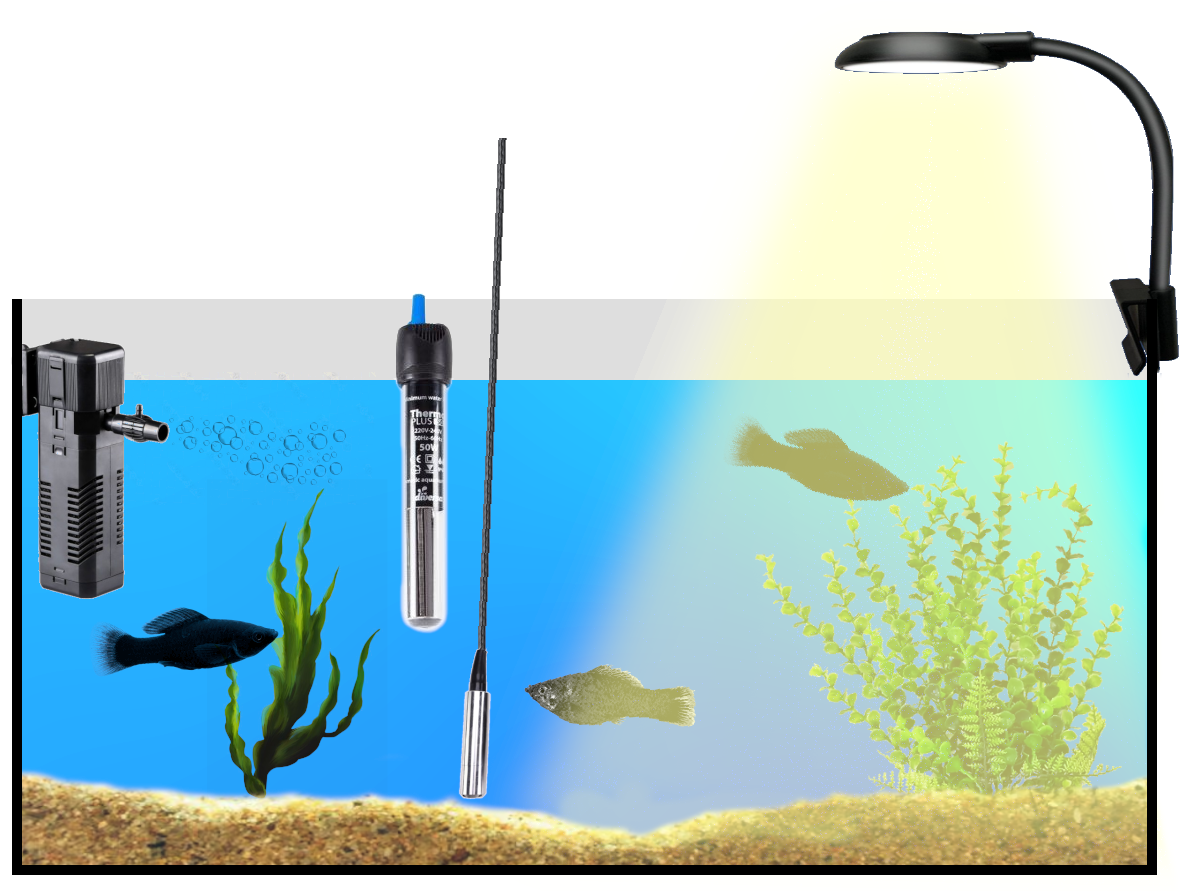
\includegraphics[width=\columnwidth]{obrazky/prezentace/vybaveni-akvaria/06-sensory.png}
				%lze vložit popisek, ale povetšinou je to v prezentaci zbytečné
				%\caption{Popisek obrázku}%
				%\label{obr:ukazka}
			\end{figure}
		\end{column}
	\end{columns}											% ukončení prostředí sloupce
\end{frame}


% endregion

%%%%%%%%%%%%%
\begin{frame}[fragile]
	\frametitle{Průzkum trhu -- existující řešení automatizace}
	
	\begin{columns}[T] 								% prostředí sloupce s umístěním nahoře
		\begin{column}{0.5\textwidth}		% první sloupec
			Nabídka:\\[1ex]
			%
			\begin{itemize}
				\item Převážně velmi komplexní systémy
				\item Firmy GHL, NeptuneSystems
			\end{itemize}

			\vspace{1.5ex}%
			Výhody:\\[1ex]
			%
			\begin{itemize}
				\item Vyhoví i náročným požadavkům
			\end{itemize}
			
			\vspace{1.5ex}%
			Nevýhody:\\[1ex]
			%
			\begin{itemize}
				\item Vysoká cena 
				\item Náročné nastavení systému
			\end{itemize}
			
		\end{column}
		%
		\begin{column}{0.5\textwidth}		% druhý sloupec
			\begin{figure}%	
				\centering
				\vspace{-0.8cm}	              % horizontální mezera
				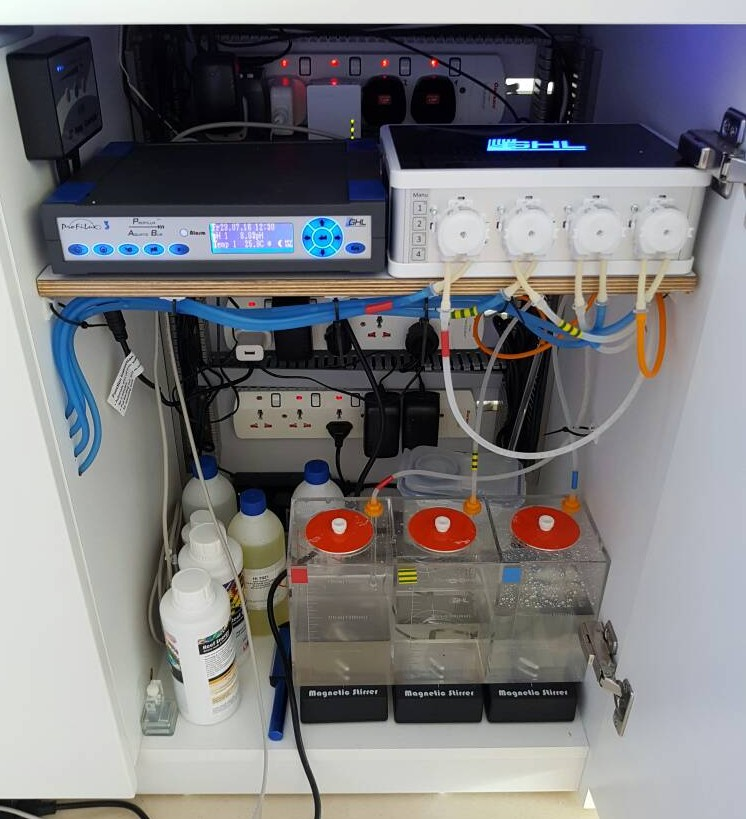
\includegraphics[width=\columnwidth]{obrazky/prezentace/ghl-from-forum.jpg}
				%lze vložit popisek, ale povetšinou je to v prezentaci zbytečné
				%\caption{Popisek obrázku}%
				%\label{obr:ukazka}
			\end{figure}
		\end{column}
	\end{columns}											% ukončení prostředí sloupce
\end{frame}

%%%%%%%%%%%%%
\begin{frame}[fragile]
	\frametitle{Průzkum trhu -- existující řešení automatizace}
	
	\begin{columns}[T] 								% prostředí sloupce s umístěním nahoře
		\begin{column}{0.5\textwidth}		% první sloupec
			Jednodušší varianty:\\[1ex]
			%
			\begin{itemize}
				\item Firma CoralVue
			\end{itemize}

			% \vspace{3ex}%
			% \begin{figure}%	
			% 	\centering
			% 	\vspace{-0.8cm}	              % horizontální mezera
			% 	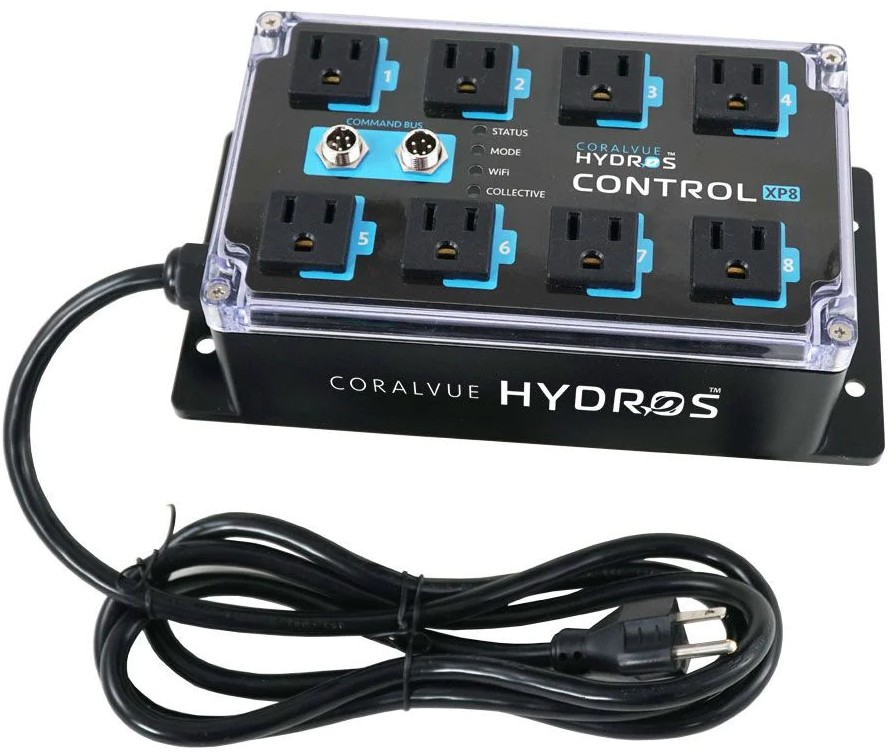
\includegraphics[width=\columnwidth]{obrazky/hydros.jpg}
			% 	%lze vložit popisek, ale povetšinou je to v prezentaci zbytečné
			% 	%\caption{Popisek obrázku}%
			% 	%\label{obr:ukazka}
			% \end{figure}
			
		\end{column}
		%
		\begin{column}{0.5\textwidth}		% druhý sloupec
			\begin{figure}%	
				\centering
				\vspace{-0.5cm}	              % horizontální mezera
				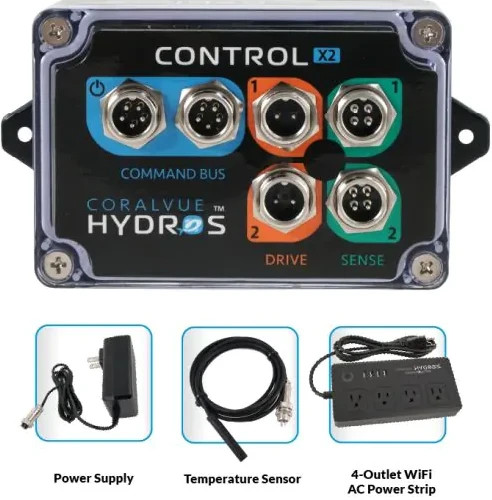
\includegraphics[width=\columnwidth]{obrazky/prezentace/hydros-x2-starter-pack.jpg}
				%lze vložit popisek, ale povetšinou je to v prezentaci zbytečné
				%\caption{Popisek obrázku}%
				%\label{obr:ukazka}
			\end{figure}
		\end{column}
	\end{columns}											% ukončení prostředí sloupce
\end{frame}

%%%%%%%%%%%%%
\begin{frame}[fragile]
	\frametitle{Návrh vlastního zařízení -- Specifikace požadavků}
	
	\begin{columns}[T] 								% prostředí sloupce s umístěním nahoře
		\begin{column}{0.8\textwidth}		% první sloupec
			Určení zařízení:\\[1ex]
			%
			\begin{itemize}
				\item Cílová skupina -- hobby akvaristé
				\begin{itemize}
					\item Malá sladkovodní akvária bez specifických potřeb
					\item Ovládání základních akčních členů a senzorů
				\end{itemize}
			\end{itemize}
			\vspace{1.5ex}%
			Klíčové parametry:\\[1ex]
			\begin{itemize}
				\item Jednoduchost instalace a obsluhy
				\item Rozšiřitenost systému
				\item Bezpečnost a spolehlivost
				\item Nízká cena
			\end{itemize}
		\end{column}
		%
		\begin{column}{0.2\textwidth}		% druhý sloupec
			\begin{figure}%	
				\centering
				\vspace{2cm}	              % horizontální mezera
				\hspace{-4cm}
				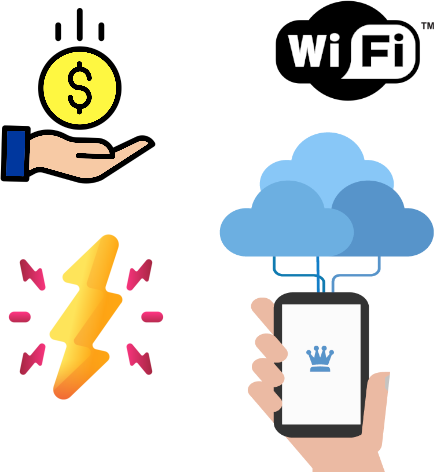
\includegraphics[width=5cm]{obrazky/prezentace/icons.png}
				%lze vložit popisek, ale povetšinou je to v prezentaci zbytečné
				%\caption{Popisek obrázku}%
				%\label{obr:ukazka}
			\end{figure}
		\end{column}
	\end{columns}											% ukončení prostředí sloupce
\end{frame}

%%%%%%%%%%%%%
\begin{frame}[fragile]
	\frametitle{Návrh vlastního zařízení -- Blokové schéma}
	\vspace{-0.8cm}
	\begin{figure}%	
		\centering
		\scalebox{0.6}
		{
		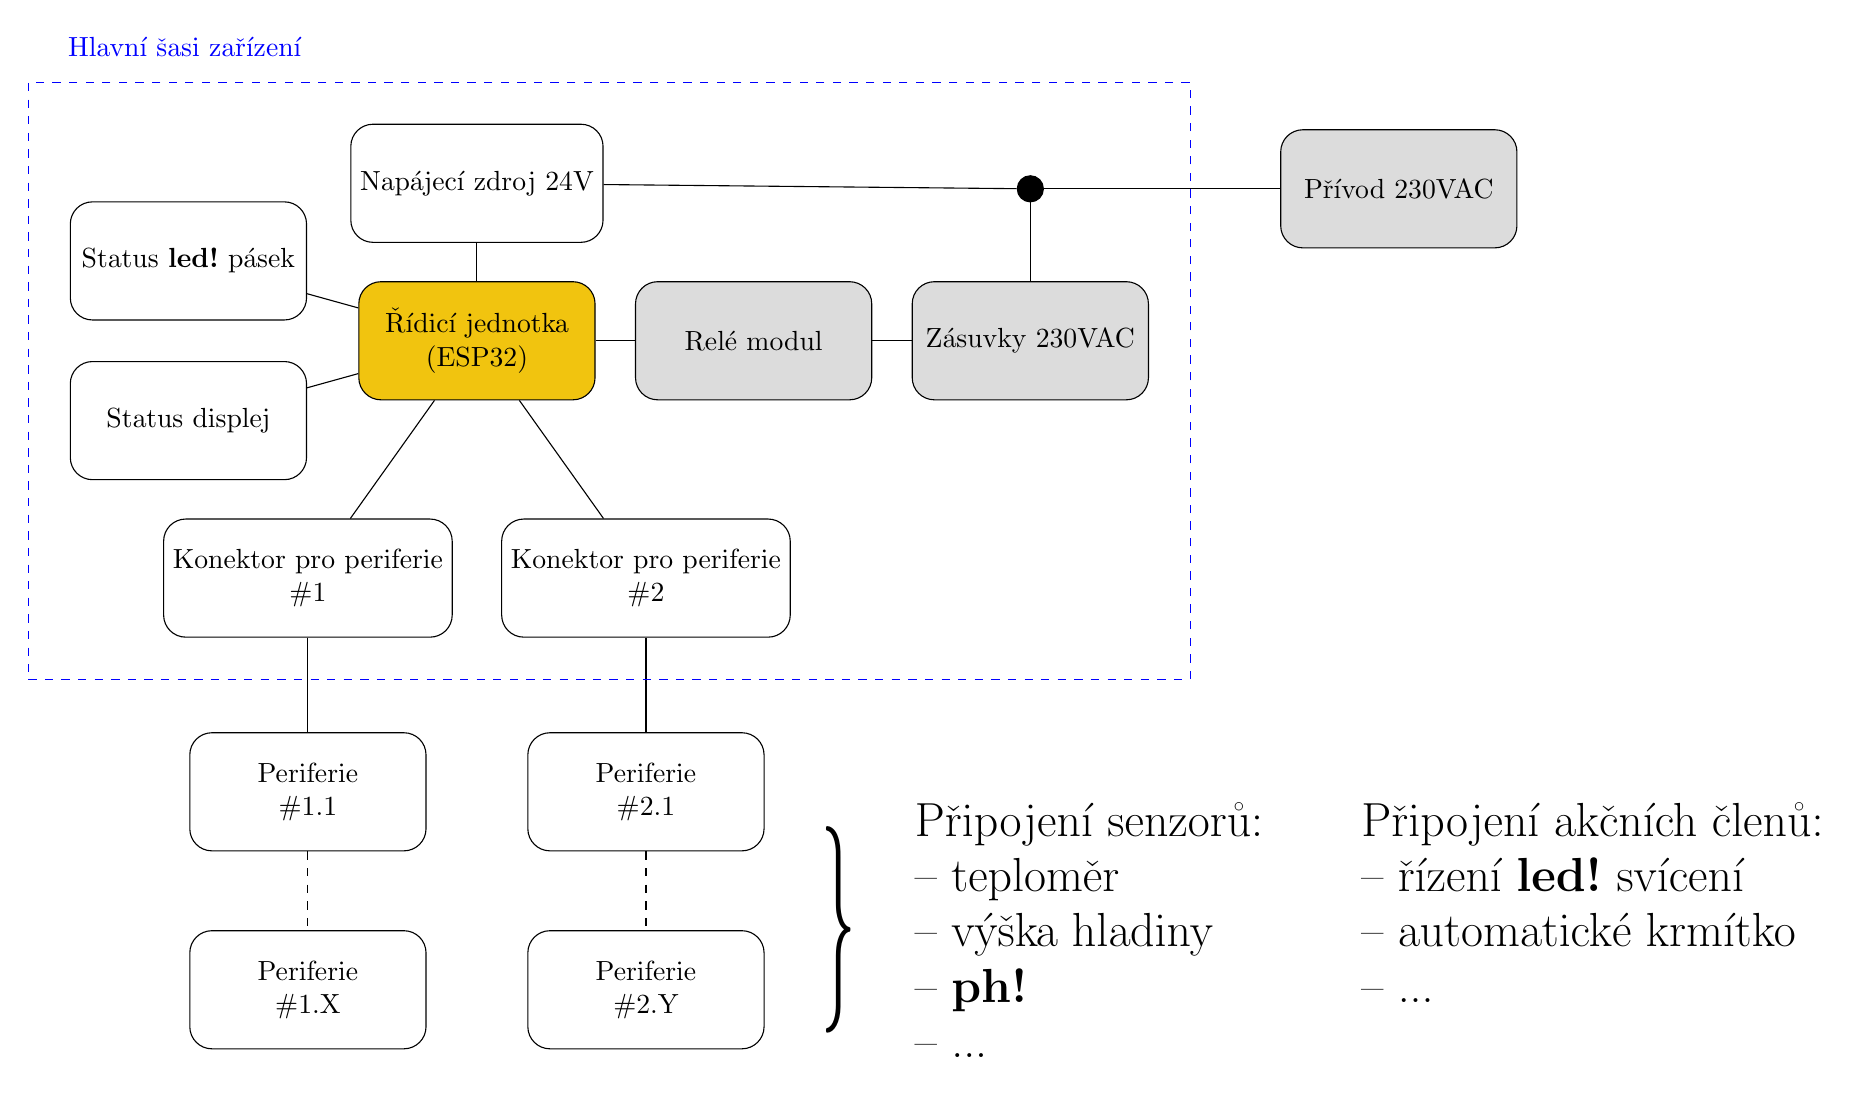
\begin{tikzpicture}[
			% scale=0.6, every node/.style={scale=0.6},
			shift={(30,30)},
			node distance=2cm,
			blok/.style={draw, rectangle, rounded corners=8pt, minimum height=1.5cm, minimum width=3cm},
			rect/.style={draw, dashed, blue, inner sep=15pt, fit={#1}},
			label/.style={blue}
		]
			% barvičky
			\definecolor{barva-silove}{RGB}{220, 220, 220}
			\definecolor{barva-ridici}{RGB}{241, 196, 15}
			% \draw (0,0) -- (4,0);
			\begin{scope}[]
				\node (napajeni) [blok, ] {Napájecí zdroj 24V};
				\node (ridici) [blok, below of = napajeni, align=center, fill=barva-ridici] {Řídicí jednotka \\ (ESP32)};
				\node (rele) [blok, right=0.5 of ridici, fill=barva-silove] {Relé modul};
				\node (zasuvky) [blok, right=0.5 of rele, fill=barva-silove] {Zásuvky 230VAC};
				\node (uzel) [style={draw, circle, minimum size=0.1cm, fill}, above=1cm of zasuvky] {};
				\node (sit) [blok, right=3 of uzel, fill=barva-silove ] {Přívod 230VAC};
				\node (display) [blok, below left=-0.5cm and 0.65cm of ridici] {Status displej};
				\node (ledstrip) [blok, above left=-0.5cm and 0.65cm of ridici] {Status \acs{led} pásek};
	
				\node (konektor1) [blok, align=center, below left=1.5cm and -1.2cm of ridici] {Konektor pro periferie \\ \#1};
				\node (konektor2) [blok, align=center, below right=1.5cm and -1.2cm of ridici] {Konektor pro periferie \\ \#2};
	
				% Periferie
				\node (per1-1) [blok, align=center, below=1.2cm of konektor1] {Periferie \\ \#1.1};
				\node (per1-x) [blok, align=center, below=1cm of per1-1] {Periferie \\ \#1.X};
			
				\node (per2-1) [blok, align=center, below=1.2cm of konektor2] {Periferie \\ \#2.1};
				\node (per2-y) [blok, align=center, below=1cm of per2-1] {Periferie \\ \#2.Y};
	
				% Popisek
				\node (vlastovka) [font=\fontsize{35}{14}\selectfont, yscale=3,  above right=-4.2cm and 0.6cm of per2-1] {\}}; 
	
				\node (popisek1) [font=\fontsize{18}{20}\selectfont,right=0.5cm of vlastovka,yshift=0cm, align=left] {Připojení senzorů: \\ -- teploměr \\ -- výška hladiny \\ -- \acs{ph} \\ -- ...};
				\node (popisek2) [font=\fontsize{18}{20}\selectfont,right=1cm of popisek1.north east, anchor=north west, align=left] {Připojení akčních členů: \\ -- řízení \acs{led} svícení \\ -- automatické krmítko \\ -- ...};
				% \node (popisek3) [below=1cm of popisek2.south west, anchor=south west, align=left] {...};
	
				% Spojovací linie
				\draw[-] (sit) -- (uzel);
				\draw[-] (uzel) -- (napajeni);
				\draw[-] (uzel) -- (zasuvky);
				\draw[-] (napajeni) -- (ridici);
				\draw[-] (ridici) -- (napajeni);
				\draw[-] (ridici) -- (display);
				\draw[-] (ridici) -- (ledstrip);
				\draw[-] (ridici) -- (konektor1);
				\draw[-] (ridici) -- (konektor2);
				\draw[-] (ridici) -- (rele);
				\draw[-] (rele) -- (zasuvky);
		
				\draw[-] (konektor1) -- (per1-1);
				\draw[dashed] (per1-1) -- (per1-x);
				
				\draw[-] (konektor2) -- (per2-1);
				\draw[dashed] (per2-1) -- (per2-y);
				
			
				% Obdélník, který obklopí vybrané uzly
				\node (hlavni-cast) [rect={(napajeni) (display) (ledstrip) (konektor1) (zasuvky)}] {};
				\node[label,above left=0.2cm and -3.6cm of hlavni-cast] {Hlavní šasi zařízení};
			\end{scope}
		\end{tikzpicture}
		}
	\end{figure}

	% \begin{columns}[T] 								% prostředí sloupce s umístěním nahoře
	% 	\begin{column}{0.4\textwidth}		% první sloupec
	% 		Typy:\\[2ex]
	% 		%
	% 		\begin{itemize}
	% 			\item Ponorné odporové těleso
	% 			\item Topný kabel
	% 		\end{itemize}

	% 		\vspace{4ex}%
	% 		Řízení:\\[2ex]
	% 		%
	% 		\begin{itemize}
	% 			\item Vlastní termostat 
	% 			\item 230\,V
	% 		\end{itemize}
	% 	\end{column}
	% 	%
	% 	\begin{column}{0.6\textwidth}		% druhý sloupec
			
	% 	\end{column}
	% \end{columns}											% ukončení prostředí sloupce
\end{frame}


%%%%%%%%%%%%%
\begin{frame}[fragile]
	\frametitle{Návrh vlastního zařízení -- Periferie}
		Periferie = samostatný blok připojený na sběrnici:\\[1ex]
		%
		\begin{itemize}
			\item Vlastní \acs{mcu} a regulátor napětí
			\item Obvody pro připojení konkrétního senzoru / akčního členu 
			\item Napájení pro náročnější součásti (např. osvětlení)
		\end{itemize}
		\vspace{1.5ex}%
		%
		Struktura:\\[1ex]
		\begin{itemize}
			\item Obecná \acs{dps} + dceřinná deska
			\begin{itemize}
				\item Urychlení vývoje
			\end{itemize}
		\end{itemize}

\end{frame}

%%%%%%%%%%%%%
\begin{frame}[fragile]
	\frametitle{Návrh vlastního zařízení -- Datová komunikace}
	Návrh ze semestrální práce:
	\begin{figure}[h!]
		\centering
		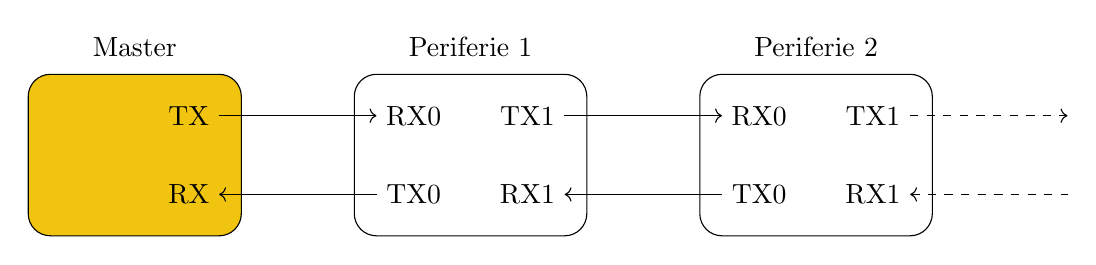
\begin{tikzpicture}[
			rect/.style={draw, inner sep=8pt, rounded corners=8pt, fit=#1},
			label/.style={black}
		]
			% barvičky
			\definecolor{barva-silove}{RGB}{220, 220, 220}
			\definecolor{barva-ridici}{RGB}{241, 196, 15}
	
			% Master device
			\node (master-tx) [] {TX};
			\node (master-rx) [below of= master-tx] {RX};
			\node (master-fitter) [left=0.6cm of master-tx] {XX};

			\node (first-rect) [rect={(master-rx) (master-tx) (master-fitter)}, fill=barva-ridici] {};
			\node[label,above=0.1cm of first-rect] {Master};
			\node at (master-tx) {TX}; %  prasárna, ale z-index nejde a nechce se mi řešit
			\node at (master-rx) {RX}; %  prasárna, ale z-index nejde a nechce se mi řešit

			
			% First device
			\node (first-rx0) [right=2cm of master-tx] {RX0};
			\node (first-tx0) [below of= first-rx0] {TX0};
			\draw[->] (master-tx) -- (first-rx0);
			\draw[<-] (master-rx) -- (first-tx0);
			\node (first-tx1) [right=0.5cm of first-rx0] {TX1};
			\node (first-rx1) [below of= first-tx1] {RX1};

			\node (first-rect) [rect={(first-rx0) (first-rx1)}] {};
			\node[label,above=0.1cm of first-rect] {Periferie 1};
			
			% % Second device
			\node (second-rx0) [right=2cm of first-tx1] {RX0};
			\node (second-tx0) [below of= second-rx0] {TX0};
			\draw[->] (first-tx1) -- (second-rx0);
			\draw[<-] (first-rx1) -- (second-tx0);
			\node (second-tx1) [right=0.5cm of second-rx0] {TX1};
			\node (second-rx1) [below of= second-tx1] {RX1};

			\node (second-rect) [rect={(second-rx0) (second-rx1)}] {};
			\node[label,above=0.1cm of second-rect] {Periferie 2};
			
			% rest
			\draw[dashed, ->] (second-tx1.east) -- ++(2cm,0);
			\draw[dashed, <-] (second-rx1.east) -- ++(2cm,0);

			% % Arrows between devices
			% \draw[->] (master) -- node[above] {TX} (device1);
			% \draw[->] (device1) -- node[above] {TX0} (device2);
			% \draw[->] (device2) -- ++(0,-1) node[below] {RX1} -- ++(-2,0) -| (master.south);
	
		\end{tikzpicture}
		% \caption{Ukázka koncepce sběrnice pro periferie.}
		\label{fig:sbernice}
	\end{figure}

		\begin{columns}[T] 								% prostředí sloupce s umístěním nahoře
		\begin{column}{0.5\textwidth}		% první sloupec
			\begin{block}{Výhody}
				\begin{itemize}
					\item Nižší cena \\
					\item Postačí UART periferie
				\end{itemize}
			\end{block}
		\end{column}
		%
		\begin{column}{0.5\textwidth}		% druhý sloupec
			\begin{alertblock}{Nevýhody}
				\begin{itemize}
					\item Nutný vlastní protokol \\
					\item Porucha snadno vyřadí více periferií
				\end{itemize}
			\end{alertblock}
		\end{column}
	\end{columns}											% ukončení prostředí sloupce
\end{frame}

%%%%%%%%%%%%%
\begin{frame}[fragile]
	\frametitle{Návrh vlastního zařízení -- Datová komunikace}
	Další varianty:\\[1ex]
	\begin{itemize}
		\item Použít průmyslovou sběrnici (\acs{can}, RS 485)
		\begin{itemize}
			\item Nutnost dalších součástek -- řadiče, kontroléry
			\item Složitější ale již existující protokol
			\item Možná kolize adres -- potřeba tento stav ošetřit
		\end{itemize}
	\end{itemize}
\end{frame}

% %%%%%%%%%%%%%
% \begin{frame}[fragile]
% 	\frametitle{Návrh vlastního zařízení -- Obecný modul periferie}
% 	Obecná \acs{dps} musí zajistit:\\[1ex]
% 	\begin{itemize}
% 		\item \acs{mcu} -- včetně napájení a programovacího rozhraní
% 		\item Datovou komunikaci 
% 		\item Vhodné ošetření konektorů
% 		\item Dutinkové lišty pro připojení dceřinné desky 
% 	\end{itemize}
% 	\vspace{2em}
% 	Dceřinná deska:\\[1ex]
% 	\begin{itemize}
% 		\item Připojení samotného senzoru / akčního členu 
% 		\begin{itemize}
% 			\item Potřebné doplňující obvody
% 			\item Měnič napětí z 24\,V pokud je potřeba 
% 		\end{itemize}
% 	\end{itemize}
% \end{frame}

%%%%%%%%%%%%%
\begin{frame}[fragile]
	\frametitle{Shrnutí práce a další postup}

	\begin{columns}[T] 								% prostředí sloupce s umístěním nahoře
		\begin{column}{0.5\textwidth}		% první sloupec
			\begin{block}{Hotovo}
				\begin{itemize}
					\item Průzkum trhu a upřesnění požadavků
					\item Návrh architektury 
					\item Schéma hlavní jednotky
					\item Výběr dalších součástí a modulů 
				\end{itemize}
			\end{block}
		\end{column}
		%
		\begin{column}{0.5\textwidth}		% druhý sloupec
			\begin{alertblock}{Následuje}
				\begin{itemize}
					\item Dokončení komunikačního rozhraní
					\item Návrh \acs{dps}
					\begin{itemize}
						\item Hlavní jednotka
						\item Obecný modul periferie
					\end{itemize}
					\item Výroba a osazení \acs{dps} 
					\item Dokončení konkrétních periferií
					\item Programování
					\item Testování
				\end{itemize}
			\end{alertblock}
		\end{column}
	\end{columns}											% ukončení prostředí sloupce
\end{frame}



% podekovani
\begin{frame}[c] 
% bez nadpisu snímku
	\frametitle{\mbox{ }}
	\begin{center}
		{\Huge Děkuji za pozornost!}
	\end{center}
\end{frame}

% zdroje
\begin{frame} [fragile]
	% bez nadpisu snímku
	\frametitle{Zdroje obrázků}
	% \hspace{-5cm}
	\begin{itemize}
		\item \url{https://www.reef2reef.com/threads/lets-see-your-ghl.258905/#post-3069873}
		\item \url{https://www.pyramidions.com/blog/the-advantages-of-using-the-cloud-technology-for-app-development/}
		\item \url{https://www.flaticon.com/free-icons/money}
		\item \url{https://www.flaticon.com/free-icons/shock}
		\item \url{https://www.coralvue.com/hydros}
	\end{itemize}			
\end{frame}

%%%%%%%%%%%%%
\begin{frame}[fragile]
	\frametitle{Návrh vlastního zařízení -- Připojení periferií}
	
			Požadavky periferií:\\[1ex]
			%
			\begin{itemize}
				\item Napájení vlastního \acs{mcu}
				\item Datová komunikace 
				\item Napájení výkonově náročnějších součástí (např. osvětlení)
			\end{itemize}
			\vspace{1.5ex}%
		%
			\begin{table}[h!]
				\centering
				\caption{Popis vodičů komunikačního rozhraní periferií.}
				\label{tab:sbernice-popis-vodicu}
				\begin{tabular}{llll}
					\toprule
					\textbf{Č.} & \textbf{Zkratka} & \textbf{Popis} & \textbf{Napětí} \\
					\midrule
					1 & 24V & Napájení z~externího zdroje, pro náročné periferie & \qty{24}{V} \\
					2 & GND0 & Zem pro výkonové napájení & \qty{0}{V}\\
					3 & 5V & Napájení pro \acs{mcu} periferií & \qty{5.2}{V}\\
					4 & GND1 & Zem pro datové linky a napájení \acs{mcu} & \qty{0}{V}\\
					5 & TX & Datový výstup & 0 až \qty{3.3}{V}\\
					6 & RX & Datový vstup & 0 až \qty{3.3}{V}\\
					\bottomrule
				\end{tabular}
			\end{table}
\end{frame}

%%%%%%%%%%%%%
\begin{frame}[fragile]
	\frametitle{Návrh vlastního zařízení -- Ochrana konektoru}
	
	\begin{figure}[h!]
		\centering
		% trim=left bottom right top
		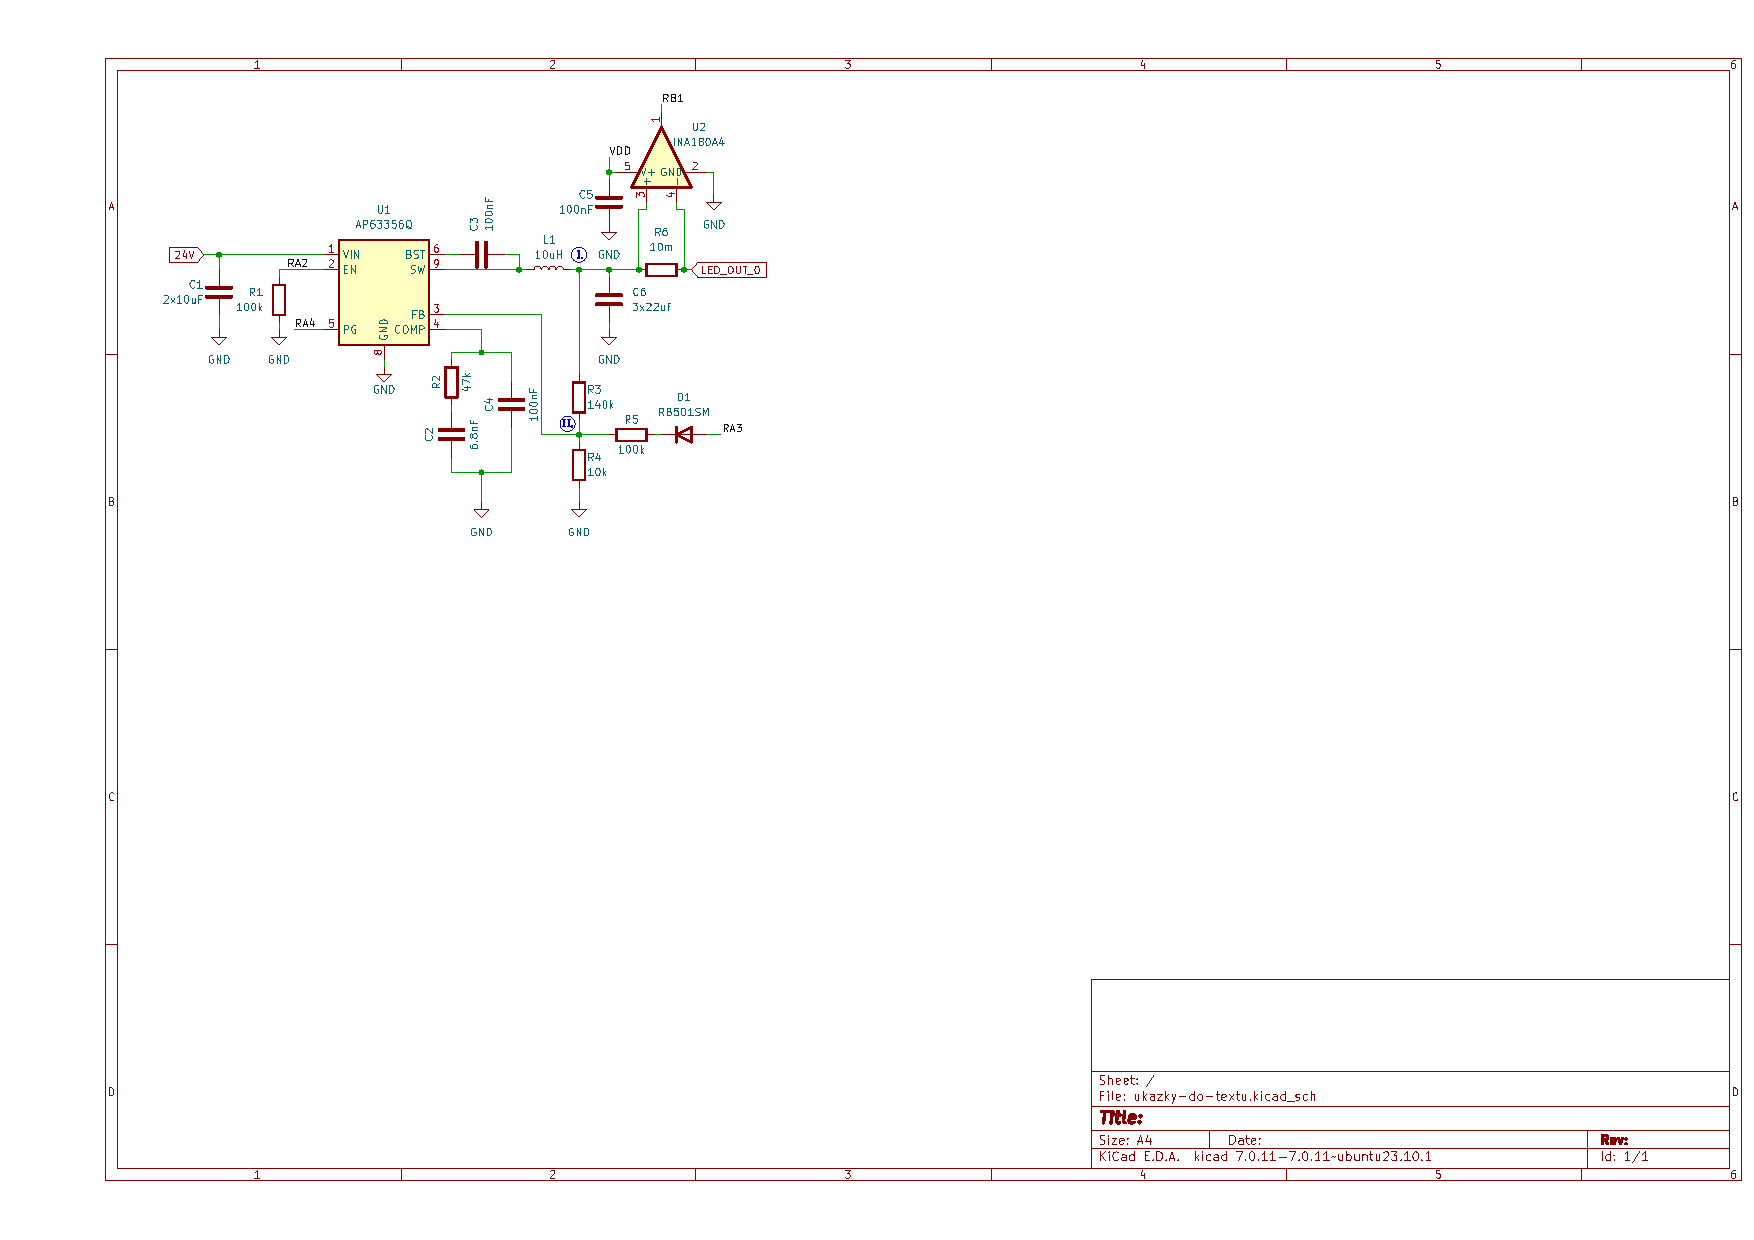
\includegraphics
		[
			width=\textwidth, 
			page=1, 
			trim=2.1cm 16cm 20cm 1.3cm, 
			clip
		]{obrazky/exportovane/ukazky-do-textu.pdf}
		% \caption{Ochrana konektorů řídicí jednotky, principiální schéma. Vytvořeno v~KiCad 7.0.}%
		\label{fig:ridici-jednotka-konektor-ochrana}
	\end{figure}

\end{frame}

\end{document}
